% Created 2020-11-16 Mon 10:02
% Intended LaTeX compiler: pdflatex
\documentclass[11pt]{article}
\usepackage[utf8]{inputenc}
\usepackage[T1]{fontenc}
\usepackage{graphicx}
\usepackage{grffile}
\usepackage{longtable}
\usepackage{wrapfig}
\usepackage{rotating}
\usepackage[normalem]{ulem}
\usepackage{amsmath}
\usepackage{textcomp}
\usepackage{amssymb}
\usepackage{capt-of}
\usepackage{hyperref}
\usepackage[russian]{babel}
\usepackage[T2A]{fontenc}
\usepackage[utf8]{inputenc}
\usepackage{minted}
\usepackage{subcaption}
\captionsetup{compatibility=false}
\author{Макаров Сергей, группа 427}
\date{\today}
\title{Контрольная работа №5}
\hypersetup{
 pdfauthor={Макаров Сергей, группа 427},
 pdftitle={Контрольная работа №5},
 pdfkeywords={},
 pdfsubject={},
 pdfcreator={Emacs 27.1 (Org mode 9.4)}, 
 pdflang={Russian}}
\begin{document}

\maketitle

\section{Задача}
\label{sec:org876dbbb}
Вычислить передаточную функцию \(f_R,Out[B_0]\) для приведённого на рисунке региона:
\begin{center}
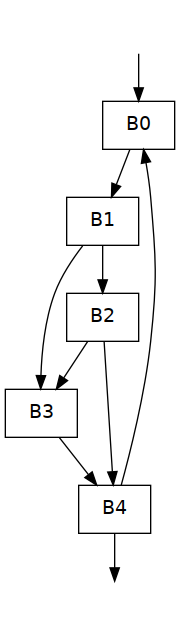
\includegraphics[height=300px]{cfg6.png}
\end{center}

Передаточные функции базовых блоков для задачи достигающих определений:
\begin{gather*}
f_0(x) = \{d_1, d_2, d_3\} \cup (x \backslash \{d_4, d_5, d_6\}) \\
f_1(x) = \{d_4, d_5\} \cup (x \backslash \{d_1, d_2, d_6\}) \\
f_2(x) = \{d_6\} \cup (x \backslash \{d_2, d_5\}) \\
f_3(x) = \{d_7\} \cup (x \backslash \{d_8\}) \\
f_4(x) = \{d_8\} \cup (x \backslash \{d_7\})
\end{gather*}
\subsection{Решение}
\label{sec:org682a74b}
В результате редукции CFG приводится к виду:
\begin{figure}[h]
\caption{Редукция CFG, шаг 1}
\label{pic:pic1}
\begin{subfigure}{0.5\textwidth}
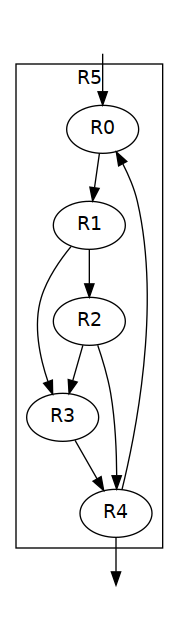
\includegraphics[height=300px]{regions5.png}

\end{subfigure}
\begin{subfigure}{0.5\textwidth}

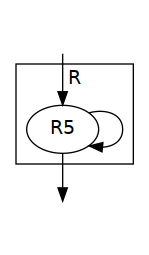
\includegraphics[height=300px]{regions6.png}

\end{subfigure}
\end{figure}
\pagebreak
\begin{center}
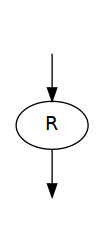
\includegraphics[height=200px]{region7.png}
\end{center}

Проходя вверх по иерархии областей, рассчитаем передаточные функции:
\begin{gather*}
f_{R_0, In[B_0]} = I, f_{R_0, Out[B_0]} = f_0, \\
f_{R_1, In[B_1]} = I, f_{R_1, Out[B_1]} = f_1, \\
f_{R_2, In[B_2]} = I, f_{R_2, Out[B_2]} = f_2, \\
f_{R_3, In[B_3]} = I, f_{R_3, Out[B_3]} = f_3, \\
f_{R_4, In[B_4]} = I, f_{R_4, Out[B_4]} = f_4, \\
f_{R_5, In[R_0]} = I, f_{R_5, Out[B_0]} = f_0, \\
f_{R_5, In[R_1]} = f_0, \\
f_{R_5, Out[B_1]} = f_1 \circ f_0 = \lambda x. \{d_3, d_4, d_5\} \cup (x \backslash \{d_1, d_2, d_4, d_5, d_6\}) = \lambda x. \{d_3, d_4, d_5\} \cup (x \backslash \{d_1, d_2, d_6\}), \\
f_{R_5, In[R_2]} = f_1 \circ f_0, \\
f_{R_5, Out[B_2]} = f_2 \circ f_1 \circ f_0 = \lambda x. \{d_3, d_4, d_6\} \cup (x \backslash \{d_1, d_2, d_5, d_6\}) = \lambda x. \{d_3, d_4, d_6\} \cup (x \backslash \{d_1, d_2, d_5\}), \\
f_{R_5, In[R_3]} = (f_1 \circ f_0) \vee (f_2 \circ f_1 \circ f_0) = \lambda x. \{d_3, d_4, d_5, d_6\} \cup (x \backslash \{d_1, d_2\}), \\
f_{R_5, Out[B_3]} = f_3 \circ ((f_1 \circ f_0) \vee (f_2 \circ f_1 \circ f_0)) = \lambda x. \{d_3, d_4, d_5, d_6, d_7\} \cup (x \backslash \{d_1, d_2, d_8\}), \\
f_{R_5, In[R_4]} = f_{R_5, Out[B_4]}, \\
f_{R_5, Out[B_4]} = f_4 \circ f_3 \circ ((f_1 \circ f_0) \vee (f_2 \circ f_1 \circ f_0)) = \lambda x. \{d_3, d_4, d_5, d_6, d_8\} \cup (x \backslash \{d_1, d_2, d_7\})
\end{gather*}
\begin{gather*}
f_{R, In[R_5]} = I, \\
f_{R, Out[B_4]} = f_{R_5, Out[B_4]} \circ f_{R_5, Out[B_4]}^* = \lambda x. \{d_3, d_4, d_5, d_6, d_8\} \cup (x \backslash \{d_1, d_2, d_7\})
\end{gather*}
\end{document}
